\documentclass{sig-alternate-05-2015}
\usepackage{graphicx}
\usepackage{amsfonts}
\usepackage{amssymb}
\usepackage{textcomp}
\usepackage{subfig}
\begin{document}
% Copyright
\setcopyright{acmcopyright}
%\setcopyright{acmlicensed}
%\setcopyright{rightsretained}
%\setcopyright{usgov}
%\setcopyright{usgovmixed}\usepackage{amsmath}


%\setcopyright{cagov}
%\setcopyright{cagovmixed}


% DOI
\doi{10.475/123_4}

% ISBN
\isbn{123-4567-24-567/08/06}

%Conference
\conferenceinfo{PLDI '13}{June 16--19, 2013, Seattle, WA, USA}

\acmPrice{\$15.00}

%
% --- Author Metadata here ---
\conferenceinfo{WOODSTOCK}{'97 El Paso, Texas USA}
%\CopyrightYear{2007} % Allows default copyright year (20XX) to be over-ridden - IF NEED BE.
%\crdata{0-12345-67-8/90/01}  % Allows default copyright data (0-89791-88-6/97/05) to be over-ridden - IF NEED BE.
% --- End of Author Metadata ---

\title{Characterizing AS-origin Conflicts }

%
% You need the command \numberofauthors to handle the 'placement
% and alignment' of the authors beneath the title.
%
% For aesthetic reasons, we recommend 'three authors at a time'
% i.e. three 'name/affiliation blocks' be placed beneath the title.
%
% NOTE: You are NOT restricted in how many 'rows' of
% "name/affiliations" may appear. We just ask that you restrict
% the number of 'columns' to three.
%
% Because of the available 'opening page real-estate'
% we ask you to refrain from putting more than six authors
% (two rows with three columns) beneath the article title.
% More than six makes the first-page appear very cluttered indeed.
%
% Use the \alignauthor commands to handle the names
% and affiliations for an 'aesthetic maximum' of six authors.
% Add names, affiliations, addresses for
% the seventh etc. author(s) as the argument for the
% \additionalauthors command.
% These 'additional authors' will be output/set for you
% without further effort on your part as the last section in
% the body of your article BEFORE References or any Appendices.

\numberofauthors{2} 
\author{
\alignauthor
Neeki Hushyar\\
       \affaddr{UMass Amherst}\\
       \email{nhushyar@cs.umass.edu}
% 2nd. author
\alignauthor
Angela Upreti\\
       \affaddr{UMass Amherst}\\
       \email{aupreti@cs.umass.edu}
}
\additionalauthors{Additional authors: John Smith (The Th{\o}rv{\"a}ld Group,
email: {\texttt{jsmith@affiliation.org}}) and Julius P.~Kumquat
(The Kumquat Consortium, email: {\texttt{jpkumquat@consortium.net}}).}
\date{30 July 1999}
% Just remember to make sure that the TOTAL number of authors
% is the number that will appear on the first page PLUS the
% number that will appear in the \additionalauthors section.

\maketitle
 \section{Abstract}\label{sec:abstract}
Broader Gateway Protocol (BGP) is an insecure protocol. According to BGPMon project twitter-feed, BGP prefix hijacks occur at a frequency of every few hours. A major indication of a BGP prefix hijack is multiple ASes announcing the same or more-specific bgp prefix but multiple AS origins does not necessarily imply a hijack. Part of the difficulty in identifying hijack as a third party is being able to filter out non-anomalous BGP origin conflicts.\\
We present an algorithm for filtering out most of the non-malicious AS origin conflicts. We automate filtering based on CDN, peering relationships, AS organization names, country registered for the AS and duration of the hijack to get a list of events that indicate whether misconfiguration or a hijack. To verify hijack, we manually check BGP-related forums and also check the BGPStream twitter-feed via the twitter API. We explain the reasons for our algorithm to have larger number of false positives and fewer false negatives. \\
From our study, we find that a very large fraction of AS origin conflict involve same country, same organization, ASes with peering relation or some form of traffic engineering. Only a few AS origin conflict incidents look malicious. During our period of study, that is April 2017, the median duration of the hijack or misconfigurarion lasted from less than \textbf{30 }mins. Most of the hijack or misconfigurations were propagated by the USA, Vietnam, Australia, India and Bangladesh. We also find that tier one destinations are the most common hijack destination and most of the hijacks are initiated my smaller autonomous systems. This matches our expectation formed according to the valley-free routing. Preference given to customer paths implies that tier 1 destinations and autonomous systems are easy to hijack.


%
% The code below should be generated by the tool at
% http://dl.acm.org/ccs.cfm
% Please copy and paste the code instead of the example below. 
%
\begin{CCSXML}
<ccs2012>
<concept>
<concept_id>10003033.10003079.10011704</concept_id>
<concept_desc>Networks~Network measurement</concept_desc>
<concept_significance>300</concept_significance>
</concept>
<concept>
<concept_id>10003033.10003083.10003014.10011617</concept_id>
<concept_desc>Networks~Firewalls</concept_desc>
<concept_significance>300</concept_significance>
</concept>
<concept>
<concept_id>10003033.10003068.10003069.10003071</concept_id>
<concept_desc>Networks~Deep packet inspection</concept_desc>
<concept_significance>100</concept_significance>
</concept>
</ccs2012>
\end{CCSXML}


%
% End generated code
%

%
%  Use this command to print the description
%
\printccsdesc

% We no longer use \terms command
%\terms{Theory}

\keywords{Border Gateway Protocol; BGP Hijack; BGPStream}
\section{Introduction}\label{sec:introduction}
  \subsection{BGPStream}
 The exterior gateway protocol, Border Gateway Protocol (BGP) is used to exchange reachability information among routers in different autonomous systems. BGP is a path vector protocol and BGP routers send path vector messages to their neighbors to advertise the reachability information. These BGP messages enable the routers to construct an autonomous system (AS) connectivity graph and make routing policy decisions. BGP is a control plane protocol and governs how data plane forwards packets between autonomous systems. 
 \begin{figure}
	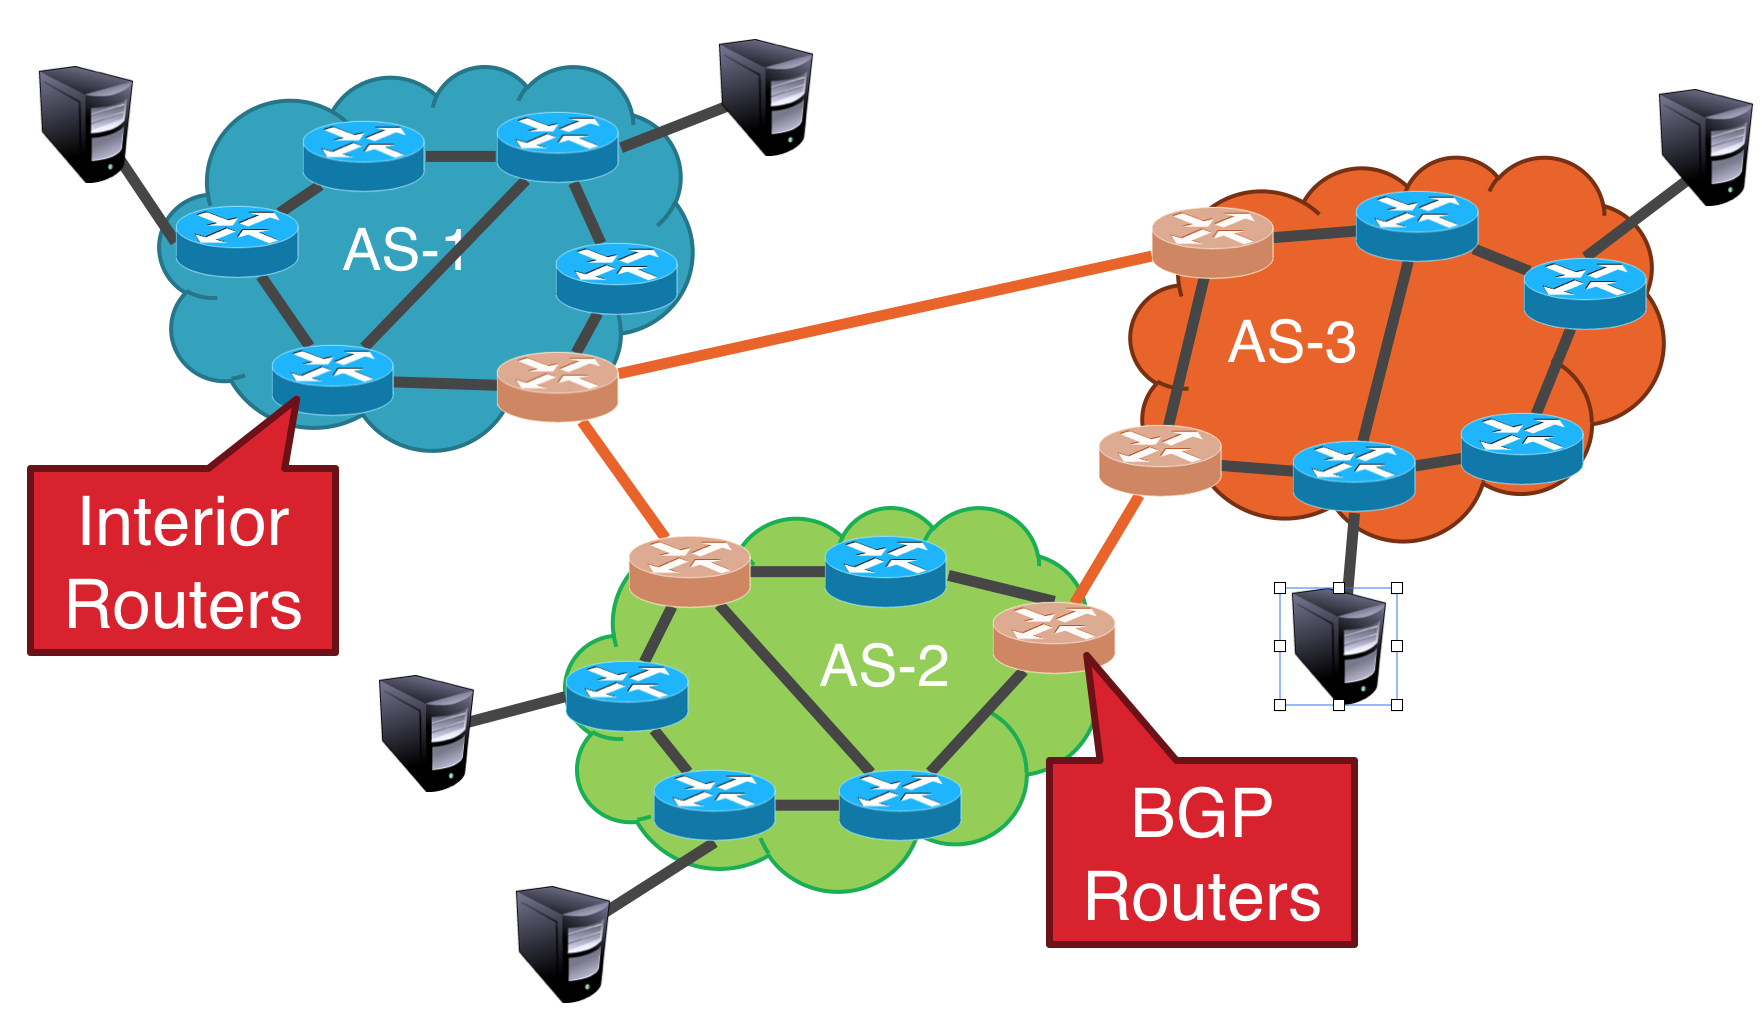
\includegraphics[width=0.5\textwidth]{Interior_and_BGP_routers.png}
	\caption{BGP routers are responsible for exchanging the path vector information. Interior routers run interior gateway protocol such as OSPF.}
\end{figure}
From the BGP routing table, a lot can be inferred about the internet topology and the peering agreements between different autonomous systems. BGP route monitors such as Route View, RIPE NCC, OpenBMP, BGPMon have made arrangements with some regional ISPs to get a dump of their RIB tables and updates to the tables. Route View monitors output RIB of participating ASes every two hours and RIPE outputs RIB every 8 hours\cite{orsini_bgpstream:_2016}. In addition to the RIB table, the monitors also output the updates to the routing table at a higher frequency. BGPStream provides a framework to analyze live and historical BGP data collected bu these monitors.  
\subsection{Anomalies in the BGP Data}
With the structure of the internet changing from hierarchical to flat, the pattern in which the autonomous systems announce prefixes has started to change. Multiple ASes announcing the same BGP prefix is no longer considered an anomaly. Emergence of CDNs has resulted in the same prefix being announced in different countries. Big organizations own multiple ASes hence, announce overlapping prefixes. Business relationships result in prefixes being traded among autonomous systems.\\
Multiple ASes announcing the same prefix can be due the changing structure of the internet, for traffic engineering, by accident, for censorship or it can be malicious. Pakistan Telecom's hijacking of the Youtube prefix is an example of an accidental BGP hijack \cite{alshamrani_detecting_2017}. With an intention of censoring YouTube, Pakistan Telecom announced YouTube's prefixes. However, announcing Youtube's prefixes to upstream provider resulted in global YouTube request traffic being redirected to Pakistan. Hacking groups have been known to hijack BGP prefixes to spam the users\cite{Ramachandran:2006:UNB:1159913.1159947}. Turkey government has hijacked the prefix of popular DNS server for censorship \cite{florio_bypassing_2014}.
 \section{Motivation}\label{sec:motivation}
 

 \begin{enumerate}
 \item Spamming
 \item Financial Gain 
 \item Accidental hijack
 \item State/Government sponsored
 \item Hacking Teams
 \end{enumerate}
 

Standard BGP is an inherently insecure protocol. Origin authentication and path validation protocols are not widely used. This allows for false announcements which can have a wide range of impacts. Attackers can use this to intercept traffic for the purposes of sniffing or redirection. In accidental cases, this can lead to performance degradation or denial of service when a user directs traffic down an incorrect path. Identifying conflicts and the sources of the conflicts is the first step in deciding what conflict detection and prevention mechanisms are most urgently needed.


 \section{Related Work}\label{sec:relatedwork}

In 2001, researchers conducted an experiment which identified valid and invalid BGP conflicts over 3 years. Valid conflicts were due to changes in providers and multi-homing, while invalid conflicts were a result of accidental and intentional misconfigurations \cite{colorado}. To identify whether a conflict was valid or invalid, they analyzed the duration of the conflicting announcements. The theory was that the longer the conflict lasted, the higher the chance of it being invalid. Our work, as well as those mentioned in the remainder of this section, found that monitoring duration is not sufficient to identify the cause of a conflict. However, we do use the duration to rule out possible causes for a conflict - namely, traffic engineering.

Another study, focused on the duration and relationship of conflicts over 10 years \cite{euro}. This allowed for correlation between seemingly independent conflicts. They found conflicts previously labeled as resulting from multi-homing, actually resulted from an increase in ASes used for improved connectivity. Further, the correlation revealed that most misconfigurations came from the same origin ASes. This study also considered the peering relationships between ASes announcing the same prefix blocks to further identify valid conflicts. Our analysis also considers peering relationships, as well other metrics which suggest a conflict is valid.

Several monitoring systems have been proposed to stop invalid paths from propogating, in real time. The first is BGPMon which consists of a network of monitors collect data and communicate with each other to make sure announcements are legitimate \cite{bgpmon}. The monitors alert network administrators whenever an unexpected announcement is seen for some prefix. ARTEMIS is another monitor which compares any BGP update to the history of paths for the given prefix and the length of previous prefix paths \cite{artemis}. Unexpected results prompt the monitors to check reverse paths. This is similar to checking the peering relationships in our study. A weakness of monitors, is maintaining a database of the true value of the prefixes and the corresponinding administrators.

The above works aimed to identify whether conflicts were valid or invalid. While we use overlapping metrics, we probe further to characterize the specific causes of the conflicts. Furthermore, our work identifies several CDNs, which previous methods may flag as an invalid conflict.

 \section{Methodology}\label{sec:methodology}
We analyzed a year's worth of BGP RIB data and classified instances where we saw multiple ASes announcing the same BGP prefix. We analyzed the BGP data from [.... select a data] in the hopes of identifying a few BGP hijacks. The known BGP hijacks  of this time were [..... list a few hijacks]which our method successfully  identifies. \\
The goal of this study was to understand the frequency and the duration of censorship intended or malicious BGP hijacks. In addition, we  use our data and our understanding of current socio-political situation surrounding the hijack to understand the popular motives behind BGP hijacks. Towards the end, based on our analysis of how most of the hijacks were accomplished, we recommend possible solutions to prevent accidental and malicious BGP hijacks. 
\subsection{Identifying BGP Hijack}
Identifying BGP hijacks involved a carefully filtering RIB table records. 
\begin{enumerate}
\item To identify the instances of BGP hijack, we started out by identifying the instances where we saw two different ASes announcing the same BGP prefix/es.
\item We used a python script to compare the whois records of the ASes announcing the same prefix. If the whois records indicated that the ASNs belonged to the same organization, we ruled out the instance. Large CDNs own many ASes throughout the world. CDNs may announce the same prefix in different parts of the world for traffic engineering. The hope is that the established peering arrangements lead to clients being directed to the closest CDN cache.
\item If the ASes annoucing the same prefix do not belong to the same organization, we check if they have a peering or a customer provider relationship.   We used ... DB to check the relationship between the two ASes[... need to find a tool to use]. This idea of using business relationship was inspired by OpenDNS's classification of BGP \cite{opendns_blackhat_2015}. It is likely that ASes with business relationships might have cosentually borrowed prefixes from teach other.  
\item If we find that the two ASes do not have either peer-peer or customer-provider relation, we then check the geolocation of the two ASes. We make use of the whois record again to compare the geolocation. If the geolocation do not match, then we say we have identified a hijack. 
\item We use bgpstream twitter feed as the `ground truth'. 
\end{enumerate}

\subsection{Hijack Characterization }

Based on the sociopolitical context and other information we have [...what other infor? ], we manually classify into three categories (1)Misconfiguration, (2)Political hijack for Censorship and (3)Malicious non-political hijack. 

We enumerate the specificity and the number of malicious BGP prefix announcement for each hijack. We calculate the difference in the specificity of the prefix announced by the hijacking AS and the hijacked AS. To determine if there is a cross-national involvement in these hijacks, we enumerate the number of malicious AS prefix announcement for each hijack. We study the geographic distributions of each of the malicious ASes.
We also characterize the target ASes of these hijacks. We determine whether the target selected (1)randomly/for fun , (2) for financial motive, (3) political motive .
\subsection{Hijack Duration and frequency}


 \section{Results}\label{sec:results}
 
Our results identifies the following sources of conflicting announcements:
\begin{itemize}
\item Accidental misconfiguration
\item Malicious hijack
\item International organization
\item Content delivery network
\end{itemize}

We collected data for the first hour of every day of April 2017. This resulted in just over 700,000 BGP announcements. We found 3 hijacks and 55 misconfigurations. We identified 3 international organizations, with ASes in different countries. We found that the hijacked prefixes belonged to China, Pakistan and Bangladesh. They were falsely announced as having AS origins in Vietnam, India and India, respectively.

It is important to note that misconfigurations are potentially unconfirmed hijackings. We found some interesting patterns in the misconfigurations of specific countries. Most of the Australian misconfigurations had the AS origin 4739. The United States announced incorrect ASes for prefixes spanning several continents, including Europe, Asia and Africa. We found that most of the misconfigurations announced by Vietnam, had prefixes owned by China. 

We also see a lot of conflicting announcement for traffic engineering purposes. One AS belonging to an organization would announce more specific prefix compared to the other AS of the same organization. We ignored conflicts spanning multiple neighboring countries. For example, there were several alerts of conflicts in which AS-origins were in Colombia and Brazil, or Hong Kong and China. We did not label these as conflicts, and filtered them out manually.


\section{Discussion}\label{sec:discussion}
Our findings matched our expectations. The only surprising \textbf{result was }
\subsection{Algorithm Validation}
Our algorithm successfully identified all three of the test hijacks. Thinking backwards, going in with the intention of identify the three hijacks helped us fine-tune our algorithm. In each of the three cases, our algorithm identified the intended hijacks and labeled some more incidents as `hijacks or misconfigurations'. This lead us to believe that our algorithm has a higher rate of false positives and lower rate of false negatives.\\
A major and an obvious source of false positives is the inability to automate separating malicious hijacks from accidental misconfigurations. Solutions to this would be using machine learning or mining bgp-related forum data which can be very expensive computationally. One of the limitations of our algorithm is the inability to identify malicious hijacks originating in the same country. Our algorithm filters out origin ASes in the same country as being non-threatening. Second, our algorithm filters out CDNS which means attacks target CDNs are not identified. These would be our sources of our false negatives. 
\subsection{Types of origin AS conflicts}
We found that most of the prefix origin conflicts result within the same country. This is not surprising given distribution of number of ASes by country is very asymmetric with large number of ASes belonging to countries such as Germany and the United States. As discussed previously, our algorithm calculates proportion of conflicting prefixes origins in the same country exclusive of CDNs and ASes belonging to the same organizations. Hence, the total number of conflicting ASes will be even higher \textbf{than}. 
We were expecting the proportion of CDNs to be a little higher due to the fact that we look for CDNs as the first step in our algorithm. This could be a limitation of the list of CDNs that we identify. However, we do identify twenty most popular CDNs which means the proportion of organizations owning multiple ASes is much much higher than \textbf{proportion} of organizations using CDNs. This indicates the existing potential market for CDNs. There is trend of moving content delivery towards the of the network and away from the backbone. Organizations owning multiple ASes can potentially save costs by moving non-sensitive contents to CDNs.
\subsection{Hijack Duration}
After identifying the hijack or misconfigurations events, we study the duration of hijack. Our estimation is only as correct frequency of RIB and update dumps to the BGP monitors. To get the estimate of the duration of the hijack, we calculate the difference between the time stamps of when the anomalous announcement was first recorded and when when the announcement was restored to the original announcement. It should be noted that this is only a rough estimation of the duration. 
\subsection{Location}
As per the availability of location information in the CAIDA datsets, we studied the most common country-level locations for hijacks. 
\subsection{Common destinations and attackers}
The most common destinations 
\subsection{Prevention}
 There are several suggested methods for BGP hijacking prevention. The simplest prevention method would be to only allow updates from the autonomous system which previously announced the path for a specific entity. This, however may negatively affect the availability and reachability of the end system. A compromise which increases the security of the update while maintaining availability, would be to delay the adoption of an update which originates from an unexpected AS. In order for this method to be implemented, the AS and AS-level edges which normally announce each BGP path, or blocks of paths, may need to be white listed in some sense. BGP updates would have to be monitored and processed. This mechanism allows time for an accidental update be removed before having widespread, if any affect. 
 
An inactive implementation of such system, is the Inernet Alert Registry (IAR). The IAR  maintained routing security information based on route history. Route history determined BGP prefix ownership and an alert was raised if an update pointed back to a different prefix. A danger of this implementation is that a trusted AS-level edge for a given prefix will not be flagged in the case it makes a false announcement. Further, in the case of the Pakistan hijack, the falsely announced route would not have been flagged as the specific prefix announced would have still been in the valid prefix space. The following mechanism would catch the previously mentioned updates which would avoid detection by the IAR.

The mechanism proposed in [...cite], creates a system to flag and alert prefix owners to any update which changes the origin. Further, sending alerts for every update has high overhead on both the monitor and on the BGP prefix owner.  

All the above prevention and detection mechanisms rely on data pooled from monitors, route server and registries. This data is not comprehensive of all BGP routes and prefixes on the internet and can only prevent/detect attacks which it can map a route for.
 
 
\section{Conclusion and Future Work}
Using BGPStream data, we searched for conflicting announcements. We successfully identified several BGP hijacks and/or accidental misconfigurations. In the process, we utilized CAIDA AS information to identify and filter out CDNs, international organizations and conflicts due to peering relationships from the conflicts we detected. A large portion of conflicts could be filtered our as same organization, as peers or originating in the same country. We found recognizable entities to be common hijack/misconfiguration destinations and entities with unfamiliar names, possibly stubs, to be the common hijackers/misconfigurers. The duration of hijacks had a median value of 23 minutes. We discuss the limitations of our algorithm in identifying prefix hijacks occurring in the same country and hijacks targeting a CDN. 

We note that our ability to label accidental misconfigurations is only as strong as the accuracy of the CAIDA relationships and AS data. We collect  our BGP announcements from BGPStream which allows us to gather data from various collectors including Route Views, RIPE and OpenBMP. While we have a full view of the prefixes announced by these collectors, we miss malicious activity by ASes not tracked by these collectors, or only partially tracked by these collectors. In addition, because of the changing internet topology, the CAIDA relationships and map dataset is always changing. This makes analyzing historical dataset on with a single threaded program on single computer hard. 

In process of writing python code for an algorithm that identifies historical hijacks as well as hijacks in real time, we have realized that the code needs to be very carefully designed. This is specially true if we are writing a single threaded code to be run on a single computer. Getting data from BGPStream is blocking and involves data transfer over a network. Similarly, our current code holds AS to organization mapping and memory information in memory. Given the size of the data we are looking at, this slows down our computation a lot. Running our algorithm for our data set, an hour of data for the month of April in 2017, easily takes more than 10 minutes. Time sensitive nature of identifying BGP hijacks demands that our program run fast. Therefore, an obvious future direction will be to make the code multi-threaded. Given the parallel nature of our workflow, using distributed computation in the form of a map-reduce architecture will speed up the program even more. Another obvious extension after adding distributed computing capabilities would be to use machine learning for classifying hijacks.

In addition, future studies can include following misconfigurations over time and correlating the results to the similar data from known hijacks. This would allow us to identify several hijacks that we currently classified as misconfigurations. 


%
% The following two commands are all you need in the
% initial runs of your .tex file to
% produce the bibliography for the citations in your paper.
\bibliographystyle{abbrv}
\bibliography{reference}  % sigproc.bib is the name of the Bibliography in this case
\end{document}